\newpage
\section{Diagrammi di attività}
\subsection{Introduzione}
I diagrammi di attività sono diagrammi che descrivono un processo. Il diagramma di attività modella un processo. Organizza più entità in un insieme di azioni secondo un determinato flusso.
Il gruppo ha deciso di prendere in esame tre possibili situazioni rilevanti all'interno dell'API Market.

\subsection{Diagramma di attività relativa alla ricerca di una API}
\begin{figure} [H]
	\centering
	\includegraphics[width=1.0\linewidth]{"IMG/ricerca API"}
	\caption{Diagramma di attività che descrive la ricerca di una API}
\end{figure}
\begin{itemize}
	\item \textbf{Precondizioni}: l'utente si trova all'interno dell'API Market e decide di effettuare una ricerca di una API in base ad alcuni parametri;
	\item \textbf{Postcondizioni}: l'Utente ha individuato l'API adatta al suo scopo e potrà acquistarla(vedi diagramma "Acquisto API");
	\item \textbf{Descrizione}: l'utente riempie un box di ricerca con i termini desiderati e in una nuova pagina visualizza le API corrispondenti ai parametri inseriti. Attualmente all'utente si presentano due possibili scelte: Effettuare una nuova ricerca con parametri diversi se i risultati della ricerca non soddisfano le sue aspettative oppure visualizzare la pagina dedicata ad una API. All'interno di una API si presentano tre possibili scenari: se l'utente è soddisfatto dell'API può decidere di proseguire l'acquisto, situazione descritta nel diagramma "Acquisto API" oppure ha due alternative: ritornare ai risultati della ricerca precedente o effettuare una nuova ricerca.
\end{itemize}

\newpage
\subsection{Diagramma di attività relativa all'acquisto di una API}
\begin{figure}[h]
	\centering
	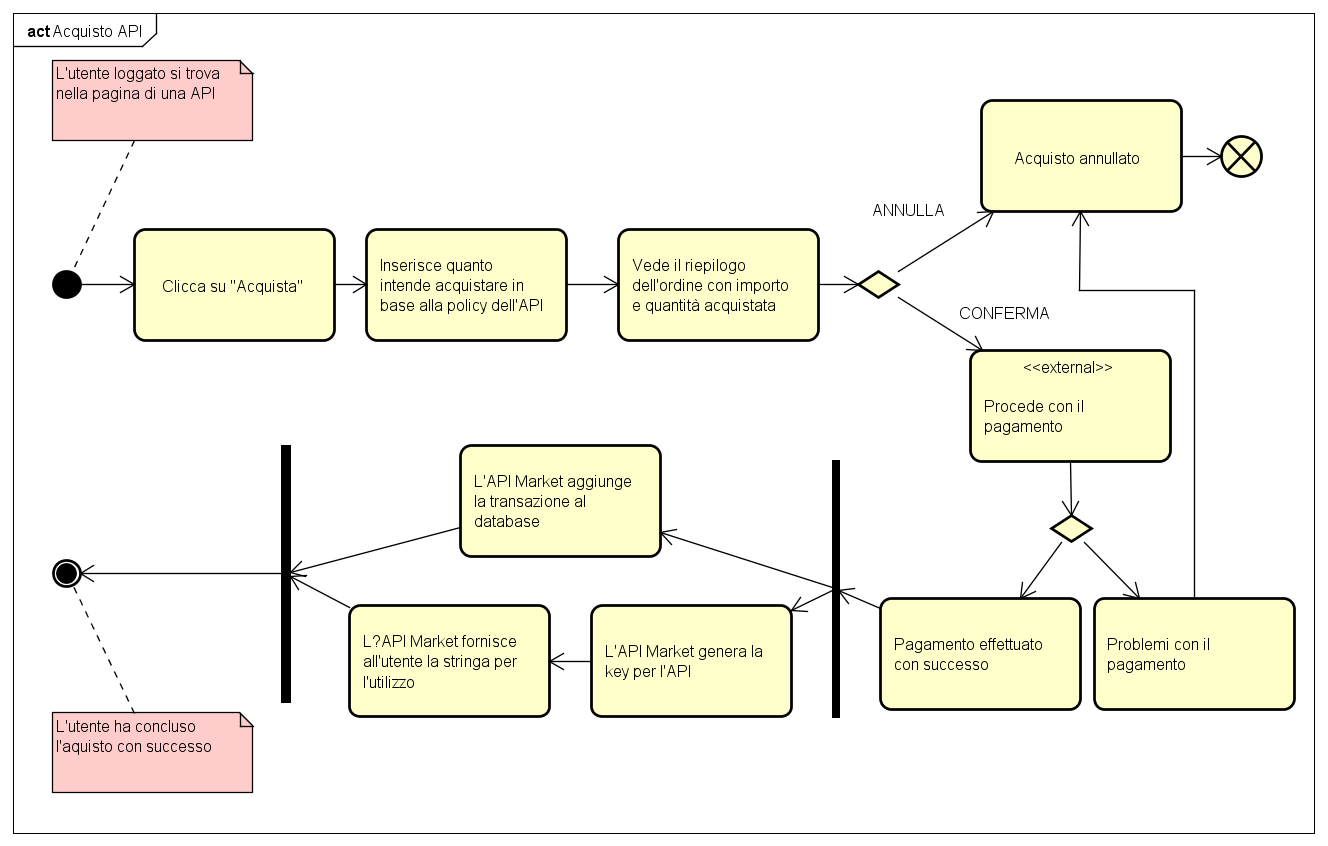
\includegraphics[width=1.0\linewidth]{IMG/Acquisto_API}
	\caption{}
	\label{fig:acquistoapi}
\end{figure}

\begin{itemize}
	\item \textbf{Precondizioni}: L'utente ha scelto un'API dal Market e vuole acquistarla;
	\item \textbf{Postcondizioni}: L'utente ha acquistato un'API e può utilizzarla;
	\item \textbf{Descrizione}: Inizialmente l'utente si trova nella pagina dell'API che desidera acquistare. Una volta cliccato su acquista inserisce la quantità che vuole acquistare in base alla policy prevista per quell'API. Successivamente vedrà un riepilogo dell'acquisto, contenente importo in euro e la quantità espressa in base alla policy, ovvero il numero di chiamate, la quantità di traffico espressa in kB oppure il tempo espresso in minuti. L'utente può decidere se confermare il pagamento tramite la piattaforma Paypal oppure annullare l'ordine. Il pagamento avviene su un sito esterno ed è possibile che la transazione non vada a buon fine, quindi è previsto il caso in cui l'utente abbia problemi con il pagamento e quindi l'acquisto venga annullato. Una volta che l'acquisto è confermato, l'API Market aggiungere la transazione al database, genera la chiave e fornisce all'utente l'indirizzo e la stringa da utilizzare per chiamare l'API, terminando l'acquisto con successo. 
\end{itemize}

\newpage
\subsection{Diagramma di attività relativa all'inserimento di una API}
\begin{figure}[h]
	\centering
	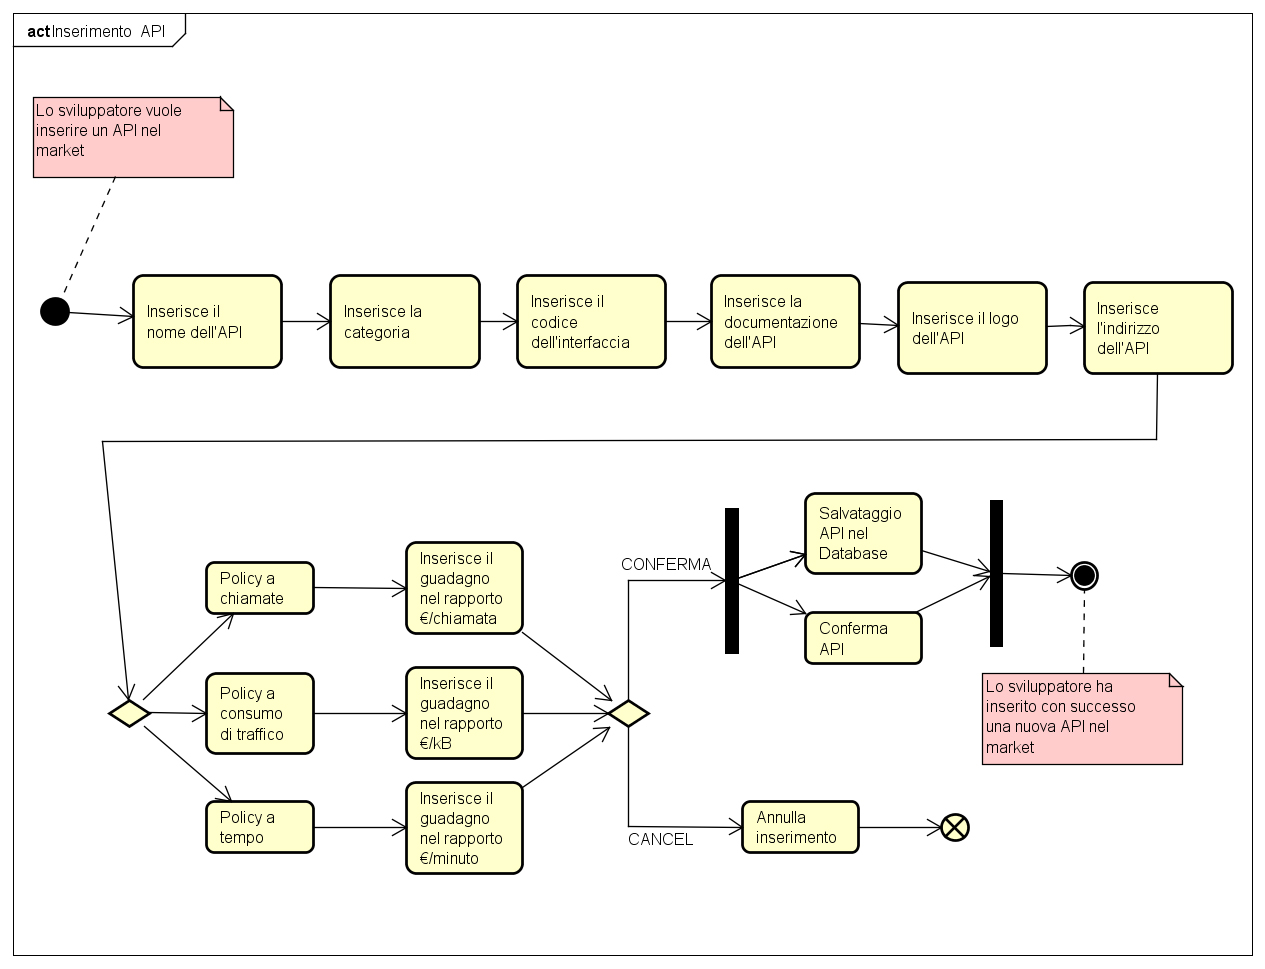
\includegraphics[width=1.0\linewidth]{IMG/Inserimento_API}
	\caption{}
	\label{fig:inserimentoapi}
\end{figure}


\begin{itemize}
	\item \textbf{Precondizioni}: L'utente ha sviluppato un'api e si trova nel suo profilo con l'intenzione di pubblicarla sul Market;
	\item \textbf{Postcondizioni}: L'utente ha aggiunto un'API al Market;
	\item \textbf{Descrizione}: L'utente si trova nel suo profilo e tramite il pulsante aggiungi API, carica una sua API sul Market. L'utente visualizza in una nuova pagina una serie di campi in cui inserire i dati richiesti per la sua API. Questi dati sono i seguenti
	\begin{itemize}
		\item Il nome dell'API;
		\item la Categoria di appartenenza dell'API;
		\item Il codice dell'interfaccia dell'API;
		\item La documentazione dell'API;
		\item Il logo dell'API;
		\item L'indirizzo dell'API;
		\item Sceglie la policy e il guadagno della sua API, ovvero:
		\begin{itemize}
			\item \textbf{Policy a chiamate}: definisce il guadagno espresso in euro per ogni chiamata da parte di un acquirente della sua API;
			\item \textbf{Policy a traffico}: definisce il guadagno espresso in euro per ogni kB trasmesso all'acquirente sua API;
			\item \textbf{Policy a tempo}: definisce il guadagno espresso in euro per ogni minuto di utilizzo da parte di un acquirente della sua API.
		\end{itemize}		
	\end{itemize}
	Successivamente può decidere se annullare il caricamento oppure confermarlo. Una volta inviata la conferma, l'API Market restituisce una conferma e salva l'API nel Database, rendendola disponibile all'acquisto da parte dei fruitori dell'API Market.
\end{itemize}


